\documentclass{beamer}
\usepackage[utf8]{inputenc}   % pour pouvoir taper les accents directement     
\usepackage{amsfonts,amssymb,amsmath}
\usepackage{tikz}
\usepackage{array}
\usepackage{calc}
\usetikzlibrary{patterns}
\usepackage[absolute,showboxes,overlay]{textpos}     
\textblockorigin{0pt}{0pt}                          
\TPshowboxesfalse  
 \usepackage{lmodern,multido}

\newcommand{\R}{\mathbb{R}}
\newcommand{\C}{\mathbb{C}}
\newcommand{\Z}{\mathbb{Z}}
\newcommand{\N}{\mathbb{N}}
\newcommand{\Q}{\mathbb{Q}}

\begin{document}
 %%%%%%%%%%%%%%%%%%%%%%%%%%%%%%%%%%%%%%%%%%%%%%%%%%%%%%%%%%%%%%%
 % Afficher le numéro de diapos 
  \addtobeamertemplate{navigation symbols}{}{ \hspace{1em}    \usebeamerfont{footline}%
    \insertframenumber/\inserttotalframenumber }
 
 %%%%%%%%%%%%%%%%%%%%%%%%%%%%%%%%%%%%%%%%%%%%%%%%%%%%%%%%%%%%%%%
\section{Introduction}
\begin{frame}{Introduction aux statistiques}
\begin{textblock*}{\textwidth}(1cm,2cm)

\begin{center}{\bf \Large Chapitre 6} \end{center}
\begin{center}{\bf \Large Statistique sur répartitions : test du $\chi^2$} \end{center}
\vspace{0.5cm}
\begin{itemize}
\item Type de données et objectifs
\item Test de conformité et d'ajustement
\item Test d'homogénéité
\item Test d'indépendance entre 2 variables
\end{itemize}

 \end{textblock*}

\end{frame}


%%%%%%%%%%%%%%%%%%%%%%%%%%%%%%%%%%%%%%%%%%%%%%%%%%%%%%%%%%%%%%%



\begin{frame}{Test du $\chi^2$}
\begin{textblock*}{\textwidth}(1cm,2cm)

\begin{center}{\bf \Large A partir de quelles données ?} \end{center}

\

\begin{itemize}
\item Populations où chaque individu peut être classé dans une catégorie $k$ (parmi 
$K$) \\
$\Rightarrow$ Nb (et proportion) d'individus dans chaque catégorie \\

\vspace{0.5cm}
\item Par exemple, sur un échantillon de taille $n$ : 
$$
\begin{array}{lcccccc}
\hline
\mbox{Catégories} & 1 & 2 & ... & K & \\
\hline
\mbox{Effectifs}  & n_1 & n_2 & ... & n_K & n \\
\mbox{Proportions}  & \frac{n_1}n & \frac{n_2}n & ...& \frac{n_K}n & 1 \\
\hline
\end{array}
$$

\end{itemize}

\end{textblock*}

\end{frame}

%%%%%%%%%%%%%%%%%%%%%%%%%%%%%%%%%%%%%%%%%%%%%%%%%%%%%%%%%%%%%%%

%%%%%%%%%%%%%%%%%%%%%%%%%%%%%%%%%%%%%%%%%%%%%%%%%%%%%%%%%%%%%%%
\begin{frame}{Test du $\chi^2$}
\begin{textblock*}{\textwidth}(1cm,2cm)

\begin{center}{\bf \Large Pour quel objectif ?} \end{center}

\begin{itemize}
\item Utiliser le test du $\chi^2$ pour :
\begin{itemize}
\item Comparer une répartition à une répartition de référence $\rightarrow$ conformité
\item Comparer deux répartitions $\rightarrow$ homogénéité
\item Vérifier si une variable aléatoire suit une certaine loi (Poisson, normale, ...)   $\rightarrow$ ajustement
\item Montrer l'indépendance d'événements (entre deux variables qualitatives)  $\rightarrow$ indépendance
\end{itemize}

\item "Généralisation" du test sur les proportions
\end{itemize}

\end{textblock*}

\end{frame}


%%%%%%%%%%%%%%%%%%%%%%%%%%%%%%%%%%%%%%%%%%%%%%%%%%%%%%%%%%%%%%%
\section{Test de conformité et d'ajustement}

\begin{frame}{Test de conformité du $\chi^2$}
\begin{textblock*}{\textwidth}(1cm,2cm)

\begin{center}{\bf \Large Exemple \\} \end{center}


\begin{itemize}
\item 3 degrés d'allergies  à l'aspirine : 

Répartition des gravités des allergies en France : 

\

\begin{center}
\begin{tabular}{|c|c|c|}
\hline
bénigne & grave & tr\`es grave \\
\hline
$45\,\%$ & $35\,\%$ & $20\,\%$\\
\hline
\end{tabular}
\end{center}

\

\item  En Lozère,  sur  150  allergiques à 
l'aspirine  : 50  allergies bénignes, 62  allergies graves et
38  allergies très graves.
\item  Lozère particulière pour l'allergie à l'aspirine ?
\end{itemize}

\end{textblock*}

\end{frame}

%%%%%%%%%%%%%%%%%%%%%%%%%%%%%%%%%%%%%%%%%%%%%%%%%%%%%%%%%%%%%%%

\begin{frame}{Test de conformité du $\chi^2$}
\begin{textblock*}{\textwidth}(1cm,2cm)

\begin{center}{\bf \Large Hypothèses} \end{center}

\begin{itemize}
\item  $\pi_1$, $\pi_2$ et $\pi_3$ les proportions théoriques des trois catégories en Lozère
\begin{itemize}
\item Sous $H_0$, on suppose que la répartition des allergiques en Lozère est similaire à celle en France. 
$$(H_0) : \pi_1=0.45, \, \pi_2=0.35 \, {\mbox { et }}  \pi_3=0.2$$

\item Sous $H_1$, la Lozère a une répartition différente : \\
\begin{center}
$(H_1)\,$ $\pi_1\neq 0.45$ \textcolor{red}{ou} $\pi_2\neq 0.35$ \textcolor{red}{ou}  $\pi_3\neq 0.2$
\end{center}
\end{itemize}
\end{itemize}

\end{textblock*}

\end{frame}

%%%%%%%%%%%%%%%%%%%%%%%%%%%%%%%%%%%%%%%%%%%%%%%%%%%%%%%%%%%%%%%

\begin{frame}{Test de conformité du $\chi^2$}
\begin{textblock*}{\textwidth}(1cm,2cm)

\begin{center}{\bf \Large Principe} \end{center}

\begin{itemize}
\item Statistique de test du $\chi^2$ : v.a. sur l'ensemble des échantillons de $n=150$ :
$$
Q(echantillon)=\sum\frac{ ({\mbox { effectif observé }} -  {\mbox { effectif théorique }})^2}
 { {\mbox { effectif théorique }}} \,.
$$
\begin{itemize}
\item {\it effectifs observés} =  effectifs $n_1$, $n_2$ et $n_3$ des 3 catégories sur l'échantillon 

\item {\it effectifs théoriques} =  effectifs attendus sous $H_0$ dans un échantillon de taille $n$ avec les proportions $\pi_1$, $\pi_2$ et $\pi_3$ \\
Pour chaque catégorie : $ n \times \pi_k$
\end{itemize}
\end{itemize}

\end{textblock*}

\end{frame}

%%%%%%%%%%%%%%%%%%%%%%%%%%%%%%%%%%%%%%%%%%%%%%%%%%%%%%%%%%%%%%%

\begin{frame}{Test de conformité du $\chi^2$}
\begin{textblock*}{\textwidth}(1cm,1.5cm)

\begin{center}{\bf \Large Principe} \end{center}

\begin{itemize}
\item  Sous $H_0$ : $Q$ suit une loi du $\chi^2$ à $K-1$ ddl
à condition que : $n\geq 30$ et $n\pi_k \geq 5$ pour tout $k$
\vspace{0.3cm}
\end{itemize}

\begin{columns}[c]
\begin{column}{5cm}
\begin{itemize}
\item $Pr(Q > \underbrace{\chi^2_{K-1 ; \alpha}}_{\downarrow} ) = \alpha$ \\
\vspace{0.2cm}
à lire dans la table des valeurs extrêmes de la loi du $\chi^2$  
\end{itemize}
\end{column}

\begin{column}{5cm}
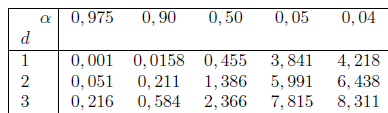
\includegraphics[scale=0.5]{images/table_chi2.png}
\end{column}
\end{columns}

\vspace{0.3cm}
\begin{itemize}
\item Zone de rejet définie par $q > \chi^2_{K-1 ; \alpha}$ \\
\end{itemize}
\end{textblock*}

\end{frame}

%%%%%%%%%%%%%%%%%%%%%%%%%%%%%%%%%%%%%%%%%%%%%%%%%%%%%%%%%%%%%%%

\begin{frame}{Test de conformité du $\chi^2$}
\begin{textblock*}{\textwidth}(1cm,2cm)

\begin{center}{\bf \Large Exemple} \end{center}
\begin{itemize}
\item $(H_0)$  vraie : $\pi_1=0.45$, $\pi_2=0.35$ et $\pi_3=0.2$

\item Vérification des conditions de validité avec les $\pi_i$ \\

\item Tableau des effectifs : \\
\vspace{0.5cm}
\small
\hspace{-1.2cm}
\begin{tabular}{|l|c|c|c|}
\hline
        & bénigne & grave & tr\`es grave\\
\hline
Effectifs observés & $n_1=50$ & $n_2=62$ & $n_3=38$ \\
\hline
Effectifs théoriques & $n\times 0.45=67.5$ & $n\times 0.35=52.5$ & $n\times 0.2=30$ \\
\hline
\end{tabular}
\\
\end{itemize}

\end{textblock*}

\end{frame}

%%%%%%%%%%%%%%%%%%%%%%%%%%%%%%%%%%%%%%%%%%%%%%%%%%%%%%%%%%%%%%%

\begin{frame}{Test de conformité du $\chi^2$}
\begin{textblock*}{\textwidth}(1cm,2cm)

\begin{center}{\bf \Large Exemple} \end{center}

\begin{itemize}
\item Calcul de q : 
$$q = \frac{(n_1 - n\times 0.45)^2}{n\times 0.45} + \frac{(n_2 - n\times 0.35)^2}{n\times 0.35}
+ \frac{(n_3 - n\times 0.2)^2}{n\times 0.2} \approx 8.39$$

\item Valeur seuil : $\chi^2_{2 ; 0.05} = 5.991$ \\
$\Rightarrow$ $q>5.99$ donc Rejet de $H_0$ \\

\item Différence significative des répartitions des degrés d'allergie à
l'aspirine de la Lozère par rapport à la France. 

\item Degré de signification : 0.02\\
\end{itemize}

%\begin{center}
%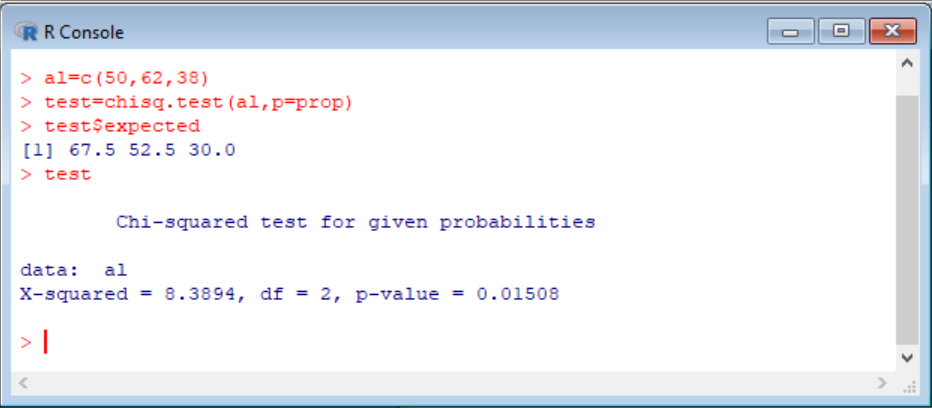
\includegraphics[width=6cm]{images/chi_conformite.png}
%\end{center}

\end{textblock*}

\end{frame}

%%%%%%%%%%%%%%%%%%%%%%%%%%%%%%%%%%%%%%%%%%%%%%%%%%%%%%%%%%%%%%%

\begin{frame}{Test d'ajustement du $\chi^2$}
\begin{textblock*}{\textwidth}(1cm,2cm)

\begin{center}{\bf \Large Comme le test de conformité ...} \end{center}

\begin{itemize}
\item Objectif : Vérifier si une v.a. suit une certaine loi \\
$\Rightarrow$ On compare une répartition à une répartition de référence \\
(comme pour le test de conformité)

\item Proportions théoriques calculées à partir de la loi

\item Principe du test inchangé\\

\begin{center}{\bf \Large ... ou presque} \end{center}

\item Si paramètre de la loi inconnu à estimer : \\
\begin{itemize}
\item On utilise les données de l'échantillon pour estimer le paramètre de la loi ({\it par ex à partir de P(X=0)})
\item Q suit une loi du $\chi^2$ à $K-\mathbf{2}$ ddl. 
\end{itemize}
\end{itemize}

\end{textblock*}

\end{frame}

%%%%%%%%%%%%%%%%%%%%%%%%%%%%%%%%%%%%%%%%%%%%%%%%%%%%%%%%%%%%%%%
\section{Test d'homogénéité} 

\begin{frame}{Test d'homogénéité du $\chi^2$}
\begin{textblock*}{\textwidth}(1cm,2cm)

\begin{center}{\bf \Large Test d'homogénéité } \end{center}
\begin{center}
Comparaison de $C$ répartitions dans $K$ catégories \end{center}

\vspace{0.5cm}
Exemple : Préférences en matière de vin :

\begin{itemize}
\item  Midi-Pyrénées :  110  préfèrent le rouge, 
70  le blanc et 20  le rosé
\item Languedoc :  120  préfèrent le rouge, 
70  le blanc et 60  le rosé
\item Existe-t-il une différence significative entre ces deux régions ?\\
\end{itemize}
\vspace{0.5cm}
Comparaison de 2 répartitions dans 3 catégories ($C=2$, $K=3$)

\end{textblock*}

\end{frame}


%%%%%%%%%%%%%%%%%%%%%%%%%%%%%%%%%%%%%%%%%%%%%%%%%%%%%%%%%%%%%%%

\begin{frame}{Test d'homogénéité du $\chi^2$}
\begin{textblock*}{\textwidth}(1cm,1.5cm)

\begin{center}{\bf \Large Hypothèses} \end{center}

\begin{itemize}
\item  Midi-Pyrénées : \\
$\pi_1$ : proportion théorique qui préfèrent le rouge, $\pi_2$  le blanc et $\pi_3$  le rosé
\item Languedoc : \\
$\pi'_1$ proportion théorique qui préfèrent le rouge, $\pi'_2$  le blanc et $\pi'_3$ le rosé \\
\vspace{0.5cm}
\item $(H_0)$ : Pas de différence entre les 2 régions\\ 
$\pi_1=\pi'_1, \pi_2=\pi'_2 \;\; et \;\; \pi_3=\pi'_3$ \\
\vspace{0.2cm}
$(H_1)$ : Différence entre les 2 régions \\
$\pi_1\neq\pi'_1 \; ou \; \pi_2\neq\pi'_2 \; ou \; \pi_3\neq\pi'_3$\\
\end{itemize}

\end{textblock*}

\end{frame}

%%%%%%%%%%%%%%%%%%%%%%%%%%%%%%%%%%%%%%%%%%%%%%%%%%%%%%%%%%%%%%%

\begin{frame}{Test d'homogénéité du $\chi^2$}
\begin{textblock*}{\textwidth}(1cm,1.5cm)

\begin{center}{\bf \Large Principe} \end{center}
\begin{itemize}
\item Statistique de test du $\chi^2$ :
$$
Q(echantillon)=\sum\frac{ ({\mbox { effectif observé }} -  {\mbox { effectif théorique }})^2}  { {\mbox { effectif théorique }}}$$

\item Sous $H_0$ : $Q$ suit une loi du $\chi^2$ à $(K-1)(C-1)$ ddl\\
à condition que : \\
$n\geq 30$, $n'\geq 30$, $n\pi_k \geq 5$ et $n'\pi'_k \geq 5$ pour tout 
$k$

\item $Pr(Q > \chi^2_{(K-1)(C-1) ; \alpha} ) = \alpha$ \\
 
\item Zone de rejet définie par $q > \chi^2_{(K-1)(C-1) ; \alpha}$ \\

\end{itemize}

\end{textblock*}

\end{frame}

%%%%%%%%%%%%%%%%%%%%%%%%%%%%%%%%%%%%%%%%%%%%%%%%%%%%%%%%%%%%%%%

\begin{frame}{Test d'homogénéité du $\chi^2$}
\begin{textblock*}{\textwidth}(1cm,1.5cm)

\begin{center}{\bf \Large Calcul des effectifs théoriques sous $H_0$} \end{center}

\begin{itemize}

\item à partir des proportions théoriques estimées par les proportions tous échantillons confondus : $p_1$, $p_2$ et $p_3$ \\
 
\item $n$ individus de Midi-Pyrénées, effectifs $n_1$, $n_2$ et $n_3$ 

$n'$ individus du Languedoc, effectifs  $n'_1$, $n'_2$ et $n'_3$ 

\item {\it Proportions théoriques estimées} : 
$$ p_1 = \frac{n_1+n'_1}{n+n'}\approx 0.51 \quad p_2 = \frac{n_2+n'_2}{n+n'}\approx 0.31 \quad
p_3 = \frac{n_3+n'_3}{n+n'}\approx 0.18
$$

\item {\it Effectifs théoriques} :
\begin{itemize}
\item pour Midi-Pyrénées : $ n \times p_1 \hspace{0.8cm} n \times p_2 \hspace{0.8cm} n \times p_3 \;\;$
\item pour Languedoc : \hspace{0.3cm} $ n' \times p_1 \hspace{0.7cm}  n' \times p_2 \hspace{0.7cm}  n' \times p_3 \;\;$
\end{itemize}
\end{itemize}
\end{textblock*}

\end{frame}

%%%%%%%%%%%%%%%%%%%%%%%%%%%%%%%%%%%%%%%%%%%%%%%%%%%%%%%%%%%%%%%

\begin{frame}{Test d'homogénéité du $\chi^2$}
\begin{textblock*}{\textwidth}(1cm,1.5cm)

\begin{center}{\bf \Large Exemple} \end{center}

\small 

\begin{itemize}
\item Conditions de validité avec proportions estimées $p_1$, $p_2$ et $p_3$
\item Tableau des effectifs

\scriptsize
\hspace{-1cm}
\begin{tabular}{|l|c|c|c|}
\hline
        & rouge & blanc & rosé \\
\hline
Observés (Midi-Pyrénées) & $n_1=110$ & $n_2=70$ & $n_3=20$ \\
\hline
Théoriques (Midi-Pyrénées) & $n\times p_1=102 $ & $n\times p_2=62 $ 
 & $n\times p_3=36 $ \\
\hline
Observés (Languedoc) & $n'_1=120$ & $n'_2=70$ & $n'_3=60$ \\
\hline
Théoriques (Languedoc) & $n'\times p_1= 127.5$ & $n'\times p_2=77.5 $ 
& $n'\times p_3 = 45$ \\
\hline
\end{tabular}
\normalsize
\item Calcul de la statistique de test : 
\scriptsize
\begin{eqnarray*}
q & = & \frac{(n_1 - n\times p_1)^2}{n\times p_1} + \frac{(n_2 - n\times p_2)^2}{n\times p_2}
+ \frac{(n_3 - n\times p_3)^2}{n\times p_3} \\
  &    &  + \frac{(n'_1 - n'\times p_1)^2}{n'\times p_1} + \frac{(n'_2 - n'\times p_2)^2}{n'\times p_2}
+ \frac{(n'_3 - n'\times p_3)^2}{n'\times p_3}\\
  & \approx & 14.9
\end{eqnarray*}
\normalsize

\end{itemize}

\end{textblock*}

\end{frame}

%%%%%%%%%%%%%%%%%%%%%%%%%%%%%%%%%%%%%%%%%%%%%%%%%%%%%%%%%%%%%%%

\begin{frame}{Test d'homogénéité du $\chi^2$}
\begin{textblock*}{\textwidth}(1cm,2cm)

\begin{center}{\bf \Large Exemple} \end{center}

\small 
\begin{itemize}
\item Valeur seuil : $\chi^2_{(K-1)(C-1),\alpha} = \chi^2_{2,0.05} = 5.991$ \\

\item $q>5.991$ : On rejette $H_0$ \\
$\Rightarrow$ il y a bien une différence significative entre les préférences de vin des deux régions

\item Degré de signification : $0.001$
\end{itemize}

%\begin{center}
%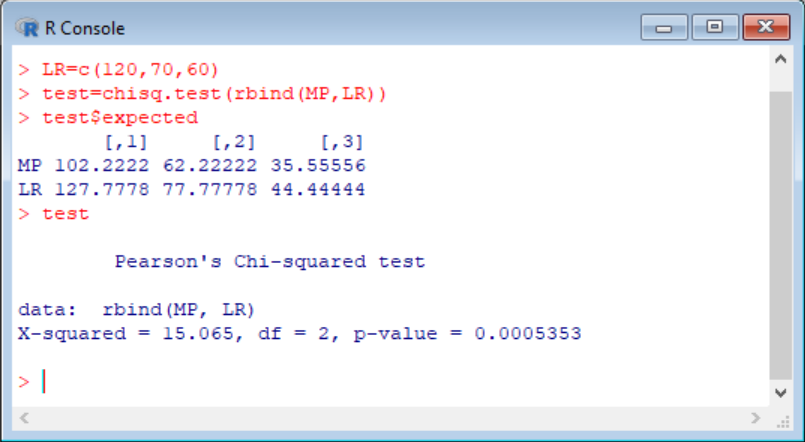
\includegraphics[width=6cm]{images/chi_homogeneite.png}
%\end{center}

\end{textblock*}

\end{frame}

%%%%%%%%%%%%%%%%%%%%%%%%%%%%%%%%%%%%%%%%%%%%%%%%%%%%%%%%%%%%%%%
\section{Test d'indépendance} 

%%%%%%%%%%%%%%%%%%%%%%%%%%%%%%%%%%%%%%%%%%%%%%%%%%%%%%%%%%%%%%%

\begin{frame}{Test d'indépendance du $\chi^2$}
\begin{textblock*}{\textwidth}(1cm,2cm)

\begin{center}{\bf \Large Test d'indépendance entre 2 variables catégorielles} \end{center}
\begin{center}
Les 2 variables catégorielles sont liées ou indépendantes ? 
\end{center}

\begin{itemize}
\item Soit un population dans laquelle chaque individu est étudié selon deux caractéristiques : 
\begin{itemize}
\item une caractéristique $X$ à $L$ catégories 
\item une caractéristique $Y$ à $C$ catégories 
\end{itemize}

\

\item Sur un échantillon de taille $n$ : 
\begin{itemize}
\item $n_{ij}$ : nombre d'individus dans les catégories $i$ et $j$ \\
($i=1,..., L$ ; $j=1,..., C$),
\end{itemize}
\end{itemize}
\end{textblock*}

\end{frame}
%%%%%%%%%%%%%%%%%%%%%%%%%%%%%%%%%%%%%%%%%%%%%%%%%%%%%%%%%%%%%%%

\begin{frame}{Test d'indépendance du $\chi^2$}
\begin{textblock*}{\textwidth}(1cm,2cm)

\begin{center}{\bf Exemple} \end{center}
\vspace{0.2cm}
137 patients atteints de cirrhose répartis selon : 
\begin{itemize}
\item le traitement reçu : placebo ou  traitement
\item le stade de gravité : 1, 2 ou 3
\end{itemize}

\small
$$
\begin{array}{lcccc}
\hline 
& \multicolumn{3}{c}{Stade} \\
& 1 & 2 & 3 & \mbox{Total} \\
\hline
\mbox{Placebo} & 13 & 29 & 26 & 68 \\
\mbox{Traitement} & 16 & 37 & 16 & 69 \\
\hline 
\mbox{Total} & 29 & 66 & 42 & 137 \\
\hline
\end{array}
$$
\end{textblock*}

\end{frame}

%%%%%%%%%%%%%%%%%%%%%%%%%%%%%%%%%%%%%%%%%%%%%%%%%%%%%%%%%%%%%%%%%%%%%%%%%%%%

\begin{frame}{Test d'indépendance du $\chi^2$}
\begin{textblock*}{\textwidth}(1cm,2cm)

\begin{center}{\bf Questions} \end{center}
\begin{itemize}
\item Le stade de gravité est-il lié au traitement ? 
\item La répartition dans les stades de gravité est-elle différente quand le patient est traité ou reçoit le placebo ? 
%\item Le traitement a-t-il un effet sur la gravité ?
\end{itemize}
$$\Downarrow$$ 

%Répartition dans les stades de gravité par groupe de traitement
%\end{textblock*}

%\end{frame}

%%%%%%%%%%%%%%%%%%%%%%%%%%%%%%%%%%%%%%%%%%%%%%%%%%%%%%%%%%%%%%%%%%%%%%%%%%%%

%\begin{frame}{Test d'indépendance du $\chi^2$}
%\begin{textblock*}{\textwidth}(1cm,1cm)

\begin{center}
\small
%$$
%\begin{array}{lcccc}
%\hline 
%& \multicolumn{3}{c}{Stade} \\
%& 1 & 2 & 3 & \mbox{Total} \\
%\hline
%\mbox{Placebo} & 13 & 29 & 26 & 68 \\
%\mbox{Traitement} & 16 & 37 & 16 & 69 \\
%\hline 
%\mbox{Total} & 29 & 66 & 42 & 137 \\
%\hline
%\end{array} $$

%$$\Downarrow$$
Répartition dans les stades de gravité par groupe de traitement
$$
\begin{array}{lcccc}
\hline 
& \multicolumn{3}{c}{Stade} \\
& 1 & 2 & 3 & \mbox{Total} \\
\hline
\mbox{Placebo} & 0.19 & 0.43 & 0.38 & 1 \\
\mbox{Traitement} & 0.23 & 0.54 & 0.23 & 1 \\
\hline 
\mbox{Tous} & 0.21 & 0.48 & 0.31 & 1 \\
\hline
\end{array}
$$
\end{center}
\end{textblock*}

\end{frame}


%%%%%%%%%%%%%%%%%%%%%%%%%%%%%%%%%%%%%%%%%%%%%%%%%%%%%%%%%%%%%%%

\begin{frame}{Test d'indépendance du $\chi^2$}
\begin{textblock*}{\textwidth}(1cm,1.5cm)

\begin{center}{\bf \Large Hypothèses} \end{center}

\begin{itemize}
\item $(H_0)$ : les 2 variables sont indépendantes \\ 
\vspace{0.2cm}
$(H_1)$ : les 2 variables ne sont pas indépendantes \

\

\item Sous $H_0$, on s'attend à ce que les répartitions par groupe de traitement soient proches de la répartition globale \\

\

\item Calcul des effectifs théoriques sous $H_0$ et comparaison avec les effectifs observés
\end{itemize}

\end{textblock*}

\end{frame}

%%%%%%%%%%%%%%%%%%%%%%%%%%%%%%%%%%%%%%%%%%%%%%%%%%%%%%%%%%%%%%%

\begin{frame}{Test d'indépendance du $\chi^2$}
\begin{textblock*}{\textwidth}(1cm,1cm)

\begin{center}{\bf \Large Calcul des effectifs théoriques sous $H_0$} \end{center}

\begin{itemize}
\item Effectifs théoriques calculés sous l'hypothèse d'indépendance : 
$$\displaystyle e_{ij} = \frac{n_{i.} \times n_{.j}}{n}$$
\begin{tabular}{ll}
où & $n_{i.}$ : nombre d'individus dans la catégorie $i$ de $X$  \\ %$n_{i.} = \sum_{j=1}^C n_{ij}$,
& $n_{.j}$ : nombre d'individus dans la catégorie $j$ de $Y$ \\ % $n_{.j} = \sum_{i=1}^L n_{ij}$,
& $n$ : nombre total d'individus dans l'échantillon \\ % $n = \sum_{i=1}^L \sum_{j=1}^C n_{ij}$.
\end{tabular}

\

%\item Effectifs théoriques sur l'exemple :
\small
$$
\begin{array}{lcccc}
\hline 
& \multicolumn{3}{c}{Stade} \\
& 1 & 2 & 3 & \mbox{Total} \\
\hline
\mbox{Placebo} & 14.4 & 32.8 & 20.8 & 68 \\
\mbox{Traitement} & 14.6 & 33.2 & 21.2 & 69 \\
\hline 
\mbox{Total} & 29 & 66 & 42 & 137 \\
\hline
\end{array}
$$


\end{itemize}
\end{textblock*}

\end{frame}


%%%%%%%%%%%%%%%%%%%%%%%%%%%%%%%%%%%%%%%%%%%%%%%%%%%%%%%%%%%%%%%

\begin{frame}{Test d'indépendance du $\chi^2$}
\begin{textblock*}{\textwidth}(1cm,1.5cm)

\begin{center}{\bf \Large Principe} \end{center}
\begin{itemize}
\item Statistique de test du $\chi^2$ :
$$
Q(echantillon)=\sum\frac{ ({\mbox { effectif observé }} -  {\mbox { effectif théorique }})^2}  { {\mbox { effectif théorique }}}$$

\item Sous $H_0$ : $Q$ suit une loi du $\chi^2$ à $(K-1)(C-1)$ ddl\\
à condition que : \\
$n\geq 30$, et $e_{ij} \geq 5$ pour tout $(i,j)$

\item $Pr(Q > \chi^2_{(K-1)(C-1) ; \alpha} ) = \alpha$ \\
 
\item Zone de rejet définie par $q > \chi^2_{(K-1)(C-1) ; \alpha}$ \\

\end{itemize}

\end{textblock*}

\end{frame}


%%%%%%%%%%%%%%%%%%%%%%%%%%%%%%%%%%%%%%%%%%%%%%%%%%%%%%%%%%%%%%%

\begin{frame}{Test d'indépendance du $\chi^2$}
\begin{textblock*}{\textwidth}(1cm,1.5cm)

\begin{center}{\bf \Large Exemple} \end{center}

\small 

\begin{itemize}
\item Conditions de validité vérifiées : tous les effectifs théoriques $> 5$ 
\item Tableau des effectifs

\scriptsize
%\hspace{-1cm}
\begin{tabular}{lccc}
\hline
        & 1 & 2 & 3 \\
\hline
Observés (Placebo) & $n_{11}=13$ & $n_{21}=29$ & $n_{31}=26$ \\
Théoriques (Placebo) & $e_{11}=14.4$ & $e_{21}=32.8$ & $e_{31}=20.8$ \\
\hline
Observés (Traitement) & $n_{12}=16$ & $n_{22}=37$ & $n_{23}=16$ \\
Théoriques (Traitement) & $e_{12}=14.6$ & $e_{22}=33.2$ & $e_{23}=21.2$\\
\hline
\end{tabular}
\normalsize

\ 

\item Calcul de la statistique de test : 
%\scriptsize
$$q  = \frac{(n_{11} - e_{11})^2}{e_{11}} + ... + \frac{(n_{23} - e_{23})^2}{e_{23}} \approx 3.65
$$
\normalsize

\end{itemize}

\end{textblock*}

\end{frame}

%%%%%%%%%%%%%%%%%%%%%%%%%%%%%%%%%%%%%%%%%%%%%%%%%%%%%%%%%%%%%%%

\begin{frame}{Test d'indépendance du $\chi^2$}
\begin{textblock*}{\textwidth}(1cm,2cm)

\begin{center}{\bf \Large Exemple} \end{center}

\small 
\begin{itemize}
\item Valeur seuil : $\chi^2_{(K-1)(C-1),\alpha} = \chi^2_{2,0.05} = 5.991$ \\

\

\item $q<5.991$ : On ne rejette pas $H_0$ \\
$\Rightarrow$ l'expérience ne permet pas de mettre en évidence une dépendance significative entre les 2 variables

\

\item Degré de signification à calculer si le test est significatif
\end{itemize}

%\begin{center}
%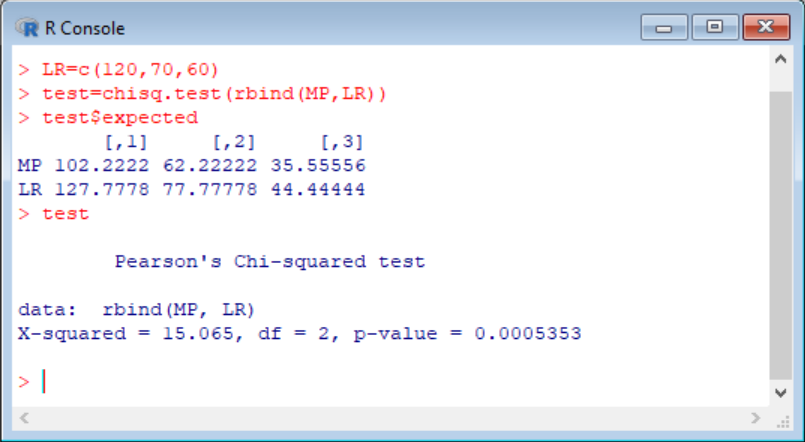
\includegraphics[width=6cm]{images/chi_homogeneite.png}
%\end{center}

\end{textblock*}

\end{frame}

%%%%%%%%%%%%%%%%%%%%%%%%%%%%%%%%%%%%%%%%%%%%%%%%%%%%%%%%%%%%%%%

\end{document}

